%%
%% This is file `main.tex',
%%
%% 1. 本模板的发布遵守 LaTeX Project Public License,使用前请认真阅读协议内容。
%%
%% 2. 本模板遵从BY-NC-SA开源协议。使用者可以对本创作进行转载、节选、混编、二次创作,
%%    但不得运用于商业目的,且使用时须进行署名,采用本创作的内容必须同样采用本协议进行授权。
%%    作为学位论文提交时可免除署名,但可以在致谢中提及。
%%
%% 3. 北京交通大学研究生院提供的 LaTeX 模板在 Overleaf 环境下几乎为不可用的状态,
%%    其版本基于清华大学Ruini Xue <xueruini@gmail.com>模板,版本较为陈旧,有较多过时代码,
%%    笔者经过若干天勘误仍无法满足正常使用需求,故重新制作了本模板。
%%
%% 4. 本模板以苯人基于「南开大学程明明老师制作的 CVPR 中文模板」制作的
%%    「东华大学本科学位论文模板」为基础,参考「北京交通大学研究生院提供的学术型硕士 LaTeX 模板」
%%    「清华大学学位论文 LaTeX 模板 v7.5.2」部分代码制作而成。部分章节以及示例文件参考自
%%    「清华大学学位论文 LaTeX 模板使用示例文档v7.5.1」。
%%
%% 5. 本模板可供给交大学生们写毕业论文及LaTeX学习参考使用,
%%    仅保证在 Overleaf 平台以 XeTeX 2024 编译器可正常使用,其余平台请自行 Debug。
%%    其格式已尽量与研究生院所规定的格式保持一致,
%%    但不保证格式审查时一定能通过,如出现格式问题,与本模板制作者概无关系。
%%
%% 6. 任何个人或组织以本模板为基础进行修改、扩展而生成的新的专用模板,
%%    请严格遵守 LaTeX Project Public License 协议。
%%    由于违犯协议而引起的任何纠纷争端均与本模板修改者无关。
%% 
%% Copyright (C) 2025 by Zeto YEUNG <yeungzeto@gmail.com>
%% 
%% This work may be distributed and/or modified under the
%% conditions of the LaTeX Project Public License, either version 1.3c
%% of this license or (at your option) any later version.
%% The latest version of this license is in
%%    https://www.latex-project.org/lppl.txt
%% and version 1.3c or later is part of all distributions of LaTeX
%% version 2008 or later.

%%%%%%%%%%%%%%%%%%% 定义学位类别 %%%%%%%%%%%%%%%
\documentclass[final,AutoFakeBold,12pt,master-academic]{bjtuthesis}
%%%%%%%%%%%%%%%%%%% 类别包含:
% 学术型硕士(master-academic)
% 专业型硕士(master-professional)
% 学术型博士(doctor-academic)
% 专业型博士(doctor-professional)
% 请修改方括号内最后一项内容,不要改变前三项!

\usepackage[pagebackref=false,breaklinks=true,colorlinks,CJKbookmarks=true]{hyperref}


%%%%%%%%%%%%%%%%%%%% 撰写时此行建议注释掉,写完后务必取消注释%%%%%%%%%%%%%%%%%%%%%
\hypersetup{linkcolor=black,citecolor=black,urlcolor=black} 
% 注释掉后可醒目查看图表章节公式引用、参考文献引用、链接引用
%%%%%%%%%%%%%%%%%%%% 撰写时此行建议注释掉,写完后务必取消注释%%%%%%%%%%%%%%%%%%%%%


% 进一步设置 hyperref 超链接的选项
\hypersetup{%
    bookmarksnumbered=true, % 书签中显示章节编号
    bookmarksopen=true, % 打开 PDF 时展开书签
    bookmarksopenlevel=1, % 默认展开到一级标题
    plainpages=false, % 允许 PDF 页面标签包含章节信息
    pdfborder=0 0 0 % 去掉超链接的边框
}

% 加载参考文献bib文件
\addbibresource{betterbib.bib}

% 定义日期
\renewcommand{\today}{\number\year 年 \number\month 月}


%%%%%%%%%%%%%%%%%%%%%%%%%%%%%%%% 定义论文信息字段
\newcommand{\ThesisTitle}{北京交通大学研究生学位论文 \LaTeX{}模板 \overleaf{} 平台专用ver.2025.3}  % 论文中文标题

\newcommand{\ThesisEngTitle}{\overleaf{} Platform-specific \LaTeX{} Template of Beijing Jiaotong University Graduate Thesis ver.2025.3}    % 论文英文标题

\newcommand{\AuthorName}{Zeto YEUNG}    % 作者姓名
\newcommand{\StudentID}{20222025}       % 作者学号
\newcommand{\Supervisor}{S. G. }        % 导师姓名
\newcommand{\SupervisorTitle}{教授}       % 导师职称
\newcommand{\DegreeType}{工学}            % 学位类别(专业学位无此行)
\newcommand{\DegreeLevel}{硕士}           % 学位级别
\newcommand{\Major}{\LaTeX{}}             % 学科专业或专业学位类别(领域)
\newcommand{\ResearchDirection}{\overleaf{}与\XeTeX{}}   % 研究方向(专业学位无此行)
\newcommand{\KeyWords}{关键词1;关键词2;关键词3}  % 中文关键词
\newcommand{\CGCN}{中图分类号Z}           % 中图分类号,可在https://www.clcindex.com/ 查询
\newcommand{\UDC}{分类号U}              % UDC分类号,可在https://udcsummary.info/php/index.php?lang=chi 查询
\newcommand{\Funding}{基金名称}         % 论文资助(填写基金名称)
\newcommand{\Lengthof}{3年}            % 学制(请如实填写)
\newcommand{\Yearof}{2025}              % 学位授予年(请如实填写)
\newcommand{\Reviewer}{评阅人姓名}       % 评阅人
\newcommand{\ChairmanofDC}{答辩委员会主席姓名}       % 答辩委员会主席
\newcommand{\MembersofDC}{答辩委员会成员姓名}       % 答辩委员会成员


\begin{document}            %%%%%%%%%%%%%%%%%%%%%%%%%%%%%% 论文开始

%%%%%%%%%%%%% 封面页、论文版权使用授权书
\coverpages
\begingroup\setbox0=\hbox{\overleaf}\endgroup % 此行内容用于预热模板中的overleaf字标,若无使用需求,可删去
\begin{center}
\vspace*{1.5cm}
\begin{figure}[H] % use float package if you want it here
  \centering
  \includesvg[width=10cm]{BJTULOGO.svg}
\end{figure}
\vskip 0.1cm
{\song\erhao\ziju{4pt}\textbf{\degreeinfo}}
\vskip 1.2cm
{\,\\\,}
{\song\xiaosan\textbf{ \ThesisTitle}}
\vskip 1cm

{\song\xiaosan\textbf{ \ThesisEngTitle}}
\vskip 3.8cm\hspace*{2cm}
\begin{minipage}[t]{5cm}\centering
\hskip -2cm{\sihao\song 作者:\ }{\sihao\song \AuthorName}
\vskip 0.6cm
\hskip -2cm{\sihao\song 导师:\ }{\sihao\song \Supervisor}
\end{minipage}

\vfill\hspace*{1cm}

\begin{minipage}[t]{5cm}
\begin{center}
{\sihao\song {\bfseries 北京交通大学}}
\vskip 0.6cm
%日期为生成当日
{\sihao \today}
\end{center}
\end{minipage}

\end{center}



\chapter*{学位论文版权使用授权书}
% \markboth{学位论文版权使用授权书}

{\xiaosi[1.3]
本学位论文作者完全了解北京交通大学有关保留、使用学位论文的规定。
特授权北京交通大学可以将学位论文的全部或部分内容编入有关数据库进行检索,提供阅览服务,
并采用影印、缩印或扫描等复制手段保存、汇编以供查阅和借阅。
同意学校向国家有关部门或机构送交论文的复印件和磁盘。
学校可以为存在馆际合作关系的兄弟高校用户提供文献传递服务和交换服务。

(保密的学位论文在解密后适用本授权说明)
\vskip 3.5cm
\begin{minipage}[t]{\textwidth}
\begin{minipage}[t]{0.45\textwidth}
学位论文作者签名:
\vskip 0.8cm
签字日期:\hspace{1cm}年\hspace{0.5cm}月\hspace{0.5cm} 日
\end{minipage}\hfill
\begin{minipage}[t]{0.45\textwidth}
导师签名:
\vskip 0.8cm
签字日期:\hspace{1cm}年\hspace{0.5cm}月\hspace{0.5cm} 日
\end{minipage}
\end{minipage}
}






%%%%%%%%%%%%% 题名页、致谢页、中英文摘要页、序、目录、图和附表清单、术语表
\ackpages
\hspace{-0.9cm}
\begin{minipage}[t][1cm]{\textwidth}\song\wuhao[1.5]
\begin{minipage}[t]{0.4\textwidth}\raggedright
学校代码:10004
\end{minipage}\hfill
\begin{minipage}[t]{0.4\textwidth}\raggedleft
密级:公开
\end{minipage}
\end{minipage}
\vskip 1.4cm

\hspace{-0.9cm}
\begin{minipage}[t][2cm]{\textwidth}\centering
{\kai\chuhao[1]\ziju{8pt} 北京交通大学}
\vskip 0.3cm
{\song\erhao[1]\ziju{6pt}  \bfseries{硕士学位论文}}
\end{minipage}

\vskip 2cm


\hspace{-0.9cm}
\hskip .6cm
\begin{minipage}[t][2cm]{.9\textwidth}\centering
{\song\xiaosan[1] 北京交通大学学术硕士学位论文 \LaTeX{}模板\\ Overleaf平台专用ver.2025.2}
\vskip 0.4cm
{\song\xiaosan[1]\ziju{4pt}  Overleaf Platform-specific \LaTeX{} Template of \\Beijing Jiaotong University Academic Master Thesis ver.2025.2}
\end{minipage}

\vskip 3.4cm

\hspace{-0.9cm}
\begin{minipage}[t][1cm]{\textwidth}\song\sihao[1]
\begin{minipage}[t]{0.5\textwidth}
作者姓名:\ Zeto YEUNG
\vskip 0.9cm						

导师姓名:\ S.G.
\vskip 0.9cm
学位类别:\  工学           			
\vskip 0.9cm
学科专业:\ \LaTeX{}  							

\end{minipage}\hfill
\begin{minipage}[t]{0.5\textwidth}
学~~~~~~~~号:\ 20222025
\vskip 0.9cm
职~~~~~~~~称:\  教授
\vskip 0.9cm
学位级别:\  硕士
\vskip 0.9cm
研究方向:\ Overleaf与\XeTeX
\end{minipage}
\end{minipage}

\vfill

\hspace{-0.9cm}
\begin{minipage}[t]{\textwidth}\centering
{\sihao\song 北京交通大学}
\vskip 0.6cm
{\sihao \today}
\end{minipage}

\null\texttt{}\relax   % 题名页
\chapter*{致谢}
\markboth{致谢}{}
放置在摘要页前,对象包括:

(1)国家科学基金,资助研究工作的奖学金基金,
合同单位,资助或支持的企业、组织或个人。

(2)协助完成研究工作和提供便利条
件的组织或个人。

(3)在研究工作中提出建议和提供帮助的人。

(4)给予转载和引
用权的资料、图片、文献、研究思想和设想的所有者。

(5)其他应感谢的组织和个
人。 
        % 致谢页

\absntocpages
\chapter*{摘要}
\markboth{摘要}{}
摘要是论文内容的高度概括,应具有独立性和自含性,即不阅读论文的全文,
就能通过摘要获得必要的信息。摘要应包括研究目的、内容、方法、结果和结论
等,重点是结果和结论。 

摘要的内容要完整、客观、准确,应做到不遗漏、不拔高、不添加。摘要应
按层次逐段简要写出,摘要在叙述研究内容、研究方法和主要结论时,除作者的
价值和经验判断可以使用第一人称外,一般使用第三人称,采用“分析了……原
因”、“研究了……”、“对……进行了探讨”“给出了……结论”等记述方法进行描
述。避免主观性的评价意见,避免对背景、目的、意义、概念和一般性(常识性)
理论叙述过多。 

摘要需采用规范的名词术语(包括地名、机构名和人名)。对个别新术语或
无中文译文的术语,可用外文或在中文译文后加括号注明外文。摘要中应尽量避
免使用图、表、化学结构式、非公知公用的符号与术语,不标注引用文献编号。 
博士学位论文摘要应包括以下几个方面的内容: 

(1)论文的研究背景及目的。简洁准确地交代论文的研究背景与意义、相
关领域的研究现状、论文所针对的关键科学问题,使读者把握论文选题的必要性
和重要性。此部分介绍不宜写得过多,一般不多于400字。 

(2)论文的主要研究方法与研究内容。介绍论文所要解决核心问题开展的
主要研究工作以及研究方法或研究手段,使读者可以了解论文的研究思路、研究
方案、研究方法或手段的合理性与先进性。 

(3)论文的主要创新成果。简要阐述论文的新思想、新观点、新技术、新
方法、新结论等主要信息,使读者可以了解论文的创新性。创新成果注意凝练和
综合,一般以2~4项为宜。 

(4)论文成果的理论和实际意义。客观、简要地介绍论文成果的理论和实
际意义,使读者可以快速获得论文的学术价值。 

摘要的字数(以汉字计),硕士学位论文一般为500~1000字,博士学位论文
一般为1000~2000字,摘要页不需写出论文题目。 

英文摘要与中文摘要的内容应完全一致,在语法、用词上应准确无误,语言
简练通顺。 

留学生的英文版硕士学位论文应有不少于3000字的“详细中文摘要”,博士学
位论文中应有不少于5000字的“详细中文摘要”。 

关键词是供检索用的主题词条,用显著的字符另起一行,排在摘要的下方。
关键词应集中体现论文特色,具有语义性,在论文中有明确的出处,并应尽量采
用《汉语主题词表》或各专业主题词表提供的规范词。每篇论文应选取3~8个关
键词。

{\bfseries 关键词:}[关键词1;关键词2;关键词3;关键词4] 




\chapter*{ABSTRACT}
\markboth{ABSTRACT}{}
The word count of the abstract (in Chinese characters) is generally 500-1000 words for master's dissertations and 1000-2000 words for doctoral dissertations.
The abstract page should not contain the title of the dissertation.

The content of the English abstract and the Chinese abstract should be identical, and the grammar and wording should be accurate, and the language should be concise and fluent.
The English abstract should be identical with the Chinese abstract in terms of grammar and diction, and the language should be concise and fluent.

The English version of the master's thesis of international students should have a detailed Chinese abstract of not less than 3000 words, and the doctoral thesis should have a detailed Chinese abstract of not less than 5000 words.
The dissertation of doctoral degree should have a "detailed Chinese abstract" of not less than 5000 words.

Keywords are the subject entries for searching, which should be placed in a separate line with prominent characters below the abstract.
Keywords should focus on the characteristics of the dissertation, be semantic, have a clear source in the dissertation, and try to use the "Chinese Theme Word List" or the "Chinese Theme Word List" as much as possible.

The keywords should focus on the characteristics of the dissertation, be semantic, have clear sources in the dissertation, and try to use the standardized words provided by Chinese Theme Word List or the theme word lists of each specialty.Each paper should choose 3-8 keywords.
Each thesis should choose 3-8 key words.


{\bfseries KEYWORDS: }[Keyword 1; Keyword 2; Keyword 3; Keyword 4]




\chapter*{序言(若有)}
\markboth{序言}{}
(可根据需要撰写或移除)学位论文的序、序言或前言,一般是作者或他人对本篇论文基本特征的简介,如说明研究工作缘起、背景、主旨、目的、意义、编写体例,以及资助、支持、协作经过等;也可以评述和对相关问题发表意见。这些内容也可以在正文绪论(引言)中说明。







   % 中英文摘要与序

\cleardoublepage    
\tableofcontents            % 目录

\cleardoublepage            % 若有图清单
\listoffigures              % 若有图清单
%%%%%%%%%%%%{(可根据需要撰写或移除)如学位论文中图表较多,应分别列出清单置于目录页之后。图的清单应有序号、图题和页码;表的清单应有序号、表题和页码。 }

\cleardoublepage            % 若有附表清单
\listoftables               % 若有附表清单
%%%%%%%%%%%%{(可根据需要撰写或移除)如学位论文中图表较多,应分别列出清单置于目录页之后。图的清单应有序号、图题和页码;表的清单应有序号、表题和页码。 }

\cleardoublepage            % 若有术语表
\nomenclature[A, 01]{$g_\mathrm{pk}{}$}{{北京地区重力加速度}
    \nomunit{\SI[group-digits=false]{9.80151}{\mathrm{kg}/\mathrm{s}^2}}}


    
\nomenclature[B,01]{BJTU}{北京交通大学}
\nomenclature[B,02]{MECE}{机械与电子控制工程学院}
\nomenclature[B,03]{RRC}{机器人研究中心}
\nomenclature[B,04]{\TeX{}}{一个优秀的排版工具,擅长于对于复杂数学符号的处理}
\nomenclature[B,05]{\LaTeX{}}{一种基于\TeX{}的排版系统}
\nomenclature[B,06]{\XeTeX{}}{一种使用Unicode的\TeX{}排版引擎,并支持一些现代字体技术}
\nomenclature[B,07]{\overleaf{}}{一个云端协作式\LaTeX{}编辑器,可用于编写和发布论文。}



\nomenclature[C]{$M$}{机构自由度}
\nomenclature[C]{$d$}{机构维数}
\nomenclature[C]{$g$}{运动副数目}
\nomenclature[C]{$f_k$}{第$k$运动副的自由度数}
\nomenclature[C]{$\xi$}{局部自由度}
   % 若有术语表
\addcontentsline{toc}{chapter}{物理量名称及符号表}
\printnomenclature          % 若有术语表

%%%%%%%%%%%%% 主体部分、参考文献、附录、结尾部分
\mainpages

\chapter{绪论}
\label{cha:intro}
\section{研究背景}
在学术论文写作过程中,排版规范和文档格式的标准化至关重要。现代科研工作者普遍采用 \LaTeX{} 作为主要的论文排版工具,尤其是在数学、物理、工程及计算机科学等领域。与传统的 WYSIWYG(所见即所得)编辑方式不同,\LaTeX{} 采用标记语言,能够实现高质量的公式排版、自动化参考文献管理、跨平台兼容性等优势 \cite{Lam1986LATEXDocument}。

近年来,云端协作工具的兴起进一步推动了 \LaTeX{} 在学术界的应用。Overleaf 作为当前最受欢迎的在线 \LaTeX{} 编辑器之一,为用户提供了多人协作、云端编译、版本管理等功能,极大提升了 \LaTeX{} 文档的可用性和易用性 \cite{OveOverleafZaiXianDeLaT}。

\textbf{本校研究生院提供的\LaTeX{}模板\cite{BeiJingJiao2014BeiJingJiaoTongDaXueBoShiShuoShiXueWeiLunWen}在\overleaf{}环境下几乎为不可用的状态},其版本基于清华大学\LaTeX{}模板,版本较为陈旧,有较多过时排版代码,笔者经过若干天勘误仍无法满足正常使用需求,故从0.5开始(以苯人基于「南开大学程明明老师制作的CVPR中文模板\cite{ChengMingMing2016ZhongWenMoBanMyCVPR}」制作的「东华大学本科学位论文模板」为基础),参考清华大学、浙江大学学位论文\cite{TUN2025LaTeXThesisTe, Wan2025ZheJiangDaXueXueWeiLunWenLaTeX}模板,重新制作了本模板。\textbf{本模板仅在\overleaf{}平台\XeTeX{} 2024 编译环境下进行测试,可供二次修改并传播。本模板遵守遵守 \LaTeX{} Project Public License,使用前请认真阅读协议内容;遵从BY-NC-SA(署名-非商业性使用-相同方式共享):使用者可以对本创作进行转载、节选、混编、二次创作,但不得运用于商业目的,且使用时须进行署名,采用本创作的内容必须同样采用本协议进行授权。作为学位论文提交时可免除署名,但可以在致谢中提及。}

\section{研究现状}
针对 \LaTeX{} 论文模板的开发,各高校和学术机构纷纷制定了符合自身格式要求的 \LaTeX{} 论文模板。例如,美国麻省理工学院(MIT) 和 加州大学伯克利分校(UC Berkeley) 分别发布了适用于本校硕博士学位论文的 \LaTeX{} 模板 \cite{MasMITthesistemp, PauPreparingYour}。在国内,清华大学、浙江大学等高校也提供了官方或非官方的 \LaTeX{} 论文模板 \cite{TUN2025LaTeXThesisTe, Wan2025ZheJiangDaXueXueWeiLunWenLaTeX}。然而,部分高校的 \LaTeX{} 论文模板更新较慢,且对 Overleaf 适配性不足,使得部分研究生仍需进行手动调整。

\section{研究目标与意义}
本研究旨在开发一款\textbf{适用于 Overleaf 平台}的《\textbf{北京交通大学学术硕士学位论文 \LaTeX{} 模板 ver.2025}》,满足学校对硕士学位论文的\textbf{格式规范},并针对 Overleaf 的特性进行优化。模板的主要目标包括:
\begin{enumerate}[itemsep=0pt,topsep=2pt,parsep=0pt]
    \item \textbf{符合北京交通大学硕士学位论文排版规范},包括封面、目录、章节标题、参考文献等格式要求;
    \item \textbf{兼容 Overleaf 云端编译环境},简化用户操作,降低使用门槛;
    \item \textbf{提供详细的模板使用说明},涵盖文档结构、数学公式、表格、插图、参考文献管理等内容,以便研究生能够快速上手并专注于论文撰写。
\end{enumerate}

本模板的开发不仅能够提高\textbf{论文排版的标准化},也能帮助学术工作者减少\textbf{格式调整}的时间成本,使其更加专注于研究本身。

[注]\quad 本章内容部分由ChatGPT 4o生成,请谨慎甄别。



  % 第一章

\chapter{论文撰写结构与规范}
\label{cha:2}

学位论文基本结构包括 5 个组成部分:前置部份、主体部份、参考文献、附
录和结尾部份。

\section{前置部份}
主要包含:
\begin{enumerate}[itemsep=0pt,topsep=2pt,parsep=0pt]
  \item 封面
  \item 学位论文版权使用授权书
  \item 题名页
  \item 致谢
  \item 摘要页
  \item 英文摘要页
  \item 序言或前言(可根据需要)
  \item 目录
  \item 图和附表清单(可根据需要)
  \item 符号、标志、缩略词、首字母缩写、计量单位、术语等的注释表(可根据需要)
\end{enumerate}

\subsection{题名 }

题名应以简明的词语,恰当、准确、科学地反映论文最重要的特定内容(一
般不超过 25 字),应中英文对照。题名通常由名词性短语构成,应尽量避免使用
不常用的缩略词、首字母缩写字、字符、代号和公式等。 

如题名内容层次很多,难以简化时,可采用题名和副题名相结合的方法,副
题名起补充、阐明题名的作用。中文的题名与副题名之间用破折号相连,英文则
用冒号相连。题名和副题名在整篇学位论文中的不同地方出现时,应保持一致。 

\subsection{致谢}

放置在摘要页前,对象包括:
\begin{enumerate}[itemsep=0pt,topsep=2pt,parsep=0pt]
  \item 国家科学基金,资助研究工作的奖学金基金,合同单位,资助或支持的企业、组织或个人。
  \item 协助完成研究工作和提供便利条件的组织或个人。
  \item 在研究工作中提出建议和提供帮助的人。
  \item 给予转载和引用权的资料、图片、文献、研究思想和设想的所有者。
  \item 其他应感谢的组织和个人。 
\end{enumerate}

\subsection{摘要与关键词}
摘要是论文内容的高度概括,应具有独立性和自含性,即不阅读论文的全文,
就能通过摘要获得必要的信息。摘要应包括研究目的、内容、方法、结果和结论
等,重点是结果和结论。 

摘要的内容要完整、客观、准确,应做到不遗漏、不拔高、不添加。摘要应
按层次逐段简要写出,摘要在叙述研究内容、研究方法和主要结论时,除作者的
价值和经验判断可以使用第一人称外,一般使用第三人称,采用“分析了……原
因”、“研究了……”、“对……进行了探讨”“给出了……结论”等记述方法进行描
述。避免主观性的评价意见,避免对背景、目的、意义、概念和一般性(常识性)
理论叙述过多。 

摘要需采用规范的名词术语(包括地名、机构名和人名)。对个别新术语或
无中文译文的术语,可用外文或在中文译文后加括号注明外文。摘要中应尽量避
免使用图、表、化学结构式、非公知公用的符号与术语,不标注引用文献编号。 
博士学位论文摘要应包括以下几个方面的内容: 

(1)论文的研究背景及目的。简洁准确地交代论文的研究背景与意义、相
关领域的研究现状、论文所针对的关键科学问题,使读者把握论文选题的必要性
和重要性。此部分介绍不宜写得过多,一般不多于400字。 

(2)论文的主要研究方法与研究内容。介绍论文所要解决核心问题开展的
主要研究工作以及研究方法或研究手段,使读者可以了解论文的研究思路、研究
方案、研究方法或手段的合理性与先进性。 

(3)论文的主要创新成果。简要阐述论文的新思想、新观点、新技术、新
方法、新结论等主要信息,使读者可以了解论文的创新性。创新成果注意凝练和
综合,一般以2~4项为宜。 

(4)论文成果的理论和实际意义。客观、简要地介绍论文成果的理论和实
际意义,使读者可以快速获得论文的学术价值。 

摘要的字数(以汉字计),硕士学位论文一般为500~1000字,博士学位论文
一般为1000~2000字,摘要页不需写出论文题目。 

英文摘要与中文摘要的内容应完全一致,在语法、用词上应准确无误,语言
简练通顺。 

留学生的英文版硕士学位论文应有不少于3000字的“详细中文摘要”,博士学
位论文中应有不少于5000字的“详细中文摘要”。 

关键词是供检索用的主题词条,用显著的字符另起一行,排在摘要的下方。
关键词应集中体现论文特色,具有语义性,在论文中有明确的出处,并应尽量采
用《汉语主题词表》或各专业主题词表提供的规范词。每篇论文应选取3~8个关
键词。

\subsection{序言或前言(可根据需要)}
学位论文的序言或前言,一般是作者对本篇论文基本特征的简介,如说明研
究工作缘起、背景、主旨、目的、意义、编写体例,以及资助、支持、协作经过
等。这些内容也可以在正文引言(绪论)中说明。 

\subsection{目录}
论文中各章节的顺序列表,包括论文中全部章、节、条三级标题及其起始页
码。排在序言或前言之后,另起页。 

\section{主体部份}
主要包含:绪论(引言)、正文及结论等部分。


\subsection{绪论(引言)}
绪论(引言)一般作为第1章。绪论(引言)应包括:本研究课题的来源、
背景及其理论意义与实际意义,国际上与课题相关研究领域的研究进展及成果,
存在的不足或有待深入研究的问题,归纳出将要开展研究的理论分析框架、研究
内容、研究程序和方法。 

绪论(引言)部分要注意对论文所引用国内外文献的准确标注\cite{BeiJingJiao2014BeiJingJiaoTongDaXueBoShiShuoShiXueWeiLunWen}。

\subsection{正文}
正文是学位论文的主要部分,必须实事求是、客观真切、准备完备、合乎逻
辑、层次分明、简练可读。论文各章之间应该前后关联,构成一个有机的整体。
论文给出的数据必须真实可靠,推理正确,结论明确,无概念性和科学性错误。
对于科学实验、计算机仿真的条件、实验过程、仿真过程等需加以叙述,然后对
结果进行分析及理论提升,避免直接给出结果、曲线和结论。引用他人研究成果
或采用他人成果时,应注明出处,不得将其与本人提出的理论分析混淆在一起。

论文主体各章后应有一节“本章小结”,实验方法或材料等章节可不写“本
章小结”。各章小结是对各章研究内容、方法与成果的简洁准确的总结与概括,也
是论文最后结论的依据。

\subsection{结论}
论文的结论是最终的、总体的结论,不是正文中每章小结的简单重复,也不
能与摘要混为一谈。结论作为学位论文正文的组成部分,单独成章,不标注引用
文献。结论应包括论文的核心观点,交待研究工作的局限,提出未来工作的意见、
建议或展望。结论应该准确、完整、明确、精炼。 

如果不能导出一定的结论,也可以没有结论而进行必要的讨论。


\section{参考文献}
参考文献应置于正文后,并另起页。 

所有被引用文献均要列入参考文献中,必须按顺序标注,但同一篇文章只用
一个序号。 

尽量引用原始文献。当不能引用原始文献时,要将二次引用文献、原始文献
同时标注。 

博士学位论文的参考文献一般不少于 100 篇,学术型硕士学位论文的参考文
献一般不少于50篇,专业硕士学位论文的参考文献一般不少于30篇,其中外文
文献一般不少于总数的1/2。参考文献中近五年的文献数一般应不少于总数的1/3,
并应有近两年的参考文献和一定数量的学位论文或专业名著。 

产品说明书、未公开发表的研究报告(著名的内部报告如PB、AD报告及著名
大公司的企业技术报告等除外)以及其它无法通过公开途径获得的文献资料通常
不宜作为参考文献引用。 

引用网上参考文献时,应注明该文献的准确网页地址,网上参考文献和各类
标准不包含在上述规定的文献数量之内。本人在攻读学位期间发表的学术论文不
应列入参考文献中。

\section{附录(可根据需要)}
附录作为主体部分的补充,可包括以下内容: 

——为了整篇论文材料的完整,但编入正文又有损于编排的条理性和逻辑性,
这一材料包括比正文更为详尽的信息、研究方法和对技术更深入的叙述,对了解
正文内容有用的补充信息等。 

——由于篇幅过大或取材于复制品而不便于编入正文的材料。

——不便于编入正文的罕见珍贵资料。 

——对一般读者并非必要阅读,但对本专业同行有参考价值的资料。 

——正文中未被引用但被阅读或具有补充信息的文献。 

——某些重要的原始数据、数学推导、结构图、统计表、计算机打印输出件等。 

\section{结尾部分}
放在附录后,对象包括:
\begin{enumerate}[itemsep=0pt,topsep=2pt,parsep=0pt]
  \item {索引(可根据需要)}
  \item {作者简历及攻读学位期间取得的研究成果} 
  \item {独创性声明} 
  \item {学位论文数据集} 
  \item {封底}
\end{enumerate}

\subsection{作者简历及攻读学位期间取得的研究成果}
作者简历包括教育经历和工作经历。 

学位论文后应列出研究生在攻读学位期间发表的与学位论文内容相关的学术
论文(含已录用的论文),与学位论文无关的学术论文不宜在此列出。攻读学位期
间所获得的科研成果、专利可单做一项分别列出。

\subsection{独创性声明 }
作者可直接下载本部分内容电子版。作者本人签署姓名。

\subsection{学位论文数据集 }
由反映学位论文主要特征的数据组成,共33项: 

A1 关键词*,A2 密级*,A3 中图分类号,A4 UDC,A5 论文资助;

B1 学位授予单位名称*,B2 学位授予单位代码*,B3 学位类别*,\\B4 学位级
别*;

C1 论文题名*,C2 并列题名,C3 论文语种*;

D1 作者姓名*,D2 学号*;

E1 培养单位名称*,E2 培养单位代码*,E3 培养单位地址,E4 邮编;

F1 学科专业*,F2 研究方向*,F3 学制*,F4 学位授予年*,F5 论文提交日
期\*;

G1 导师姓名*,G2 职称*;

H1 评阅人,H2 答辩委员会主席*,H3 答辩委员会成员;

I1 电子版论文提交格式,I2 电子版论文出版(发布)者,I3 电子版论文出
版(发布)地,I4 权限声明;

J1 论文总页数*。  % 第二章
\chapter{\LaTeX{}模板及论文撰写说明}\label{cha:3}

\section{模板基本结构与调整说明}

\subsection{模板目录与结构清单}
模板目录与结构清单如\tabref{模板目录与结构清单}所示。


\begin{table}[H]\wuhao
  \centering
  \renewcommand\arraystretch{0.8} % 行距
  \bitabcaption{模板目录与结构清单}{List of Template Catalogs and Structures}
  \begin{tabular}{ll}
    \toprule
    文件名          & 描述                         \\
    \midrule
    chapters & 论文章节存放目录  \\
    figures & 论文插图存放目录        \\
    bjtumaster.cls   & 模板文件                     \\
    main.tex & 论文主文档    \\
    betterbib.bib & 论文参考文献库(BibLaTeX)        \\
    gbt7714-numerical.bst & BibTeX 参考文献表国标样式文件    \\
    bibspacing.sty & 参考文献间距调整宏包  \\
    \bottomrule
  \end{tabular}
  \label{模板目录与结构清单}
\end{table}

使用本模板时,请在\cs{chapters}目录下删改、新增并编辑论文的章节\cs{*.tex}文件;在\cs{figures}目录下上传论文的插图;在\cs{main.tex}文件内编辑论文的整体结构;在\cs{betterbib.bib}内编辑论文引用文献的条目信息。若有需求可修改\cs{bjtumaster.cls}文件内的论文的版面结构设置。

\subsection{封面页、学位论文版权使用授权书}
需要编辑\cs{chapters}\cs{cover.tex}文件。封面页为第一部分,需\textbf{论文中、英文标题,作者,导师}四个字段。日期会自动生成,毋需编辑。学位论文版权使用授权书为第二部分,可编辑日期。签名建议脱离\LaTeX{}环境后插入或手写。

\subsection{题名页}
需要编辑\cs{chapters}\cs{cover2.tex}文件内\textbf{密级、论文中、英文标题,作者姓名、学号,导师姓名、职称,学位类别、级别,学科专业,研究方向}十一个字段。日期会自动生成,毋需编辑。

\subsection{致谢}
请在\cs{chapters}\cs{ack.tex}文件内编写。

\subsection{中英文摘要、序言}
请在\cs{chapters}\cs{abstract.tex}文件内编写。若无需序言请删除以下字段:

\begin{lstlisting}[language={[LaTeX]TeX}]
    \chapter*{序言(若有)}
    \markboth{序言}{}
    ......
\end{lstlisting}

\subsection{目录、插图清单、附表清单}
毋需手动编辑,若无插图清单、附表清单使用需求,请在\cs{main.tex}文件内删除以下字段:
\begin{lstlisting}[language={[LaTeX]TeX}]
    \cleardoublepage            % 若有图清单
    \listoffigures              % 若有图清单
    {(可根据需要撰写或移除)如学位论文中图表较多,应分别列出清单置于目录页之后。图的清单应有序
    号、图题和页码;表的清单应有序号、表题和页码。 } % 需要删除
    
    \cleardoublepage            % 若有附表清单
    \listoftables               % 若有附表清单
    {(可根据需要撰写或移除)如学位论文中图表较多,应分别列出清单置于目录页之后。图的清单应有序
    号、图题和页码;表的清单应有序号、表题和页码。 } % 需要删除
\end{lstlisting}

\subsection{术语表}
本模板提供了术语表功能,用于整理论文中的物理常数、概念与缩写、数学符号等内容。请在\cs{chapters}\cs{nomenclature.tex}文件内编辑。基本语法有三种,分别为:

\begin{lstlisting}[language={[LaTeX]TeX}]
    \nomenclature[类别]{术语}{描述}
    \nomenclature[类别, 强制排序编号]{术语}{描述}
    \nomenclature[类别, 强制排序编号]{术语}{描述}\nomunit{\SI[group-digits=false]{数值}{单位}}
\end{lstlisting}

类别包含:A:物理常数;B:概念与缩写;C:数学符号。强制排序编号为数值,如\texttt{01},可留空。对特殊物理常数可添加其常数数值与单位。

若有需求,可进入\cs{bjtumaster.cls}文件内编辑术语类别,具体定义语句为:
\begin{lstlisting}[language={[LaTeX]TeX}]
    \renewcommand\nomgroup[1]{%
        \item[\hei
        \ifstrequal{#1}{A}{物理常数}{%
        \ifstrequal{#1}{B}{概念与缩写}{%
        \ifstrequal{#1}{C}{数学符号}{}}}%
        ]\vspace{1em} % 在类别标题之后增加 1em 间距
    }
\end{lstlisting}

若无术语表使用需求,请在\cs{main.tex}文件内删除以下字段:

\begin{lstlisting}[language={[LaTeX]TeX}]
    \cleardoublepage            % 若有术语表
    \nomenclature[A, 01]{$g_\mathrm{pk}{}$}{{北京地区重力加速度}
    \nomunit{\SI[group-digits=false]{9.80151}{\mathrm{kg}/\mathrm{s}^2}}}


    
\nomenclature[B,01]{BJTU}{北京交通大学}
\nomenclature[B,02]{MECE}{机械与电子控制工程学院}
\nomenclature[B,03]{RRC}{机器人研究中心}
\nomenclature[B,04]{\TeX{}}{一个优秀的排版工具,擅长于对于复杂数学符号的处理}
\nomenclature[B,05]{\LaTeX{}}{一种基于\TeX{}的排版系统}
\nomenclature[B,06]{\XeTeX{}}{一种使用Unicode的\TeX{}排版引擎,并支持一些现代字体技术}
\nomenclature[B,07]{\overleaf{}}{一个云端协作式\LaTeX{}编辑器,可用于编写和发布论文。}



\nomenclature[C]{$M$}{机构自由度}
\nomenclature[C]{$d$}{机构维数}
\nomenclature[C]{$g$}{运动副数目}
\nomenclature[C]{$f_k$}{第$k$运动副的自由度数}
\nomenclature[C]{$\xi$}{局部自由度}
   % 若有术语表
    \printnomenclature          % 若有术语表
\end{lstlisting}

\subsection{主体部分}
请直接在\cs{chapters}目录内编辑、新建\cs{chapters0x.tex},正常标题创建方式为:
\begin{lstlisting}[language={[LaTeX]TeX}]
\chapter{章(一级)标题}
\section{节(二级)标题}
\subsection{三级标题}
\subsubsection{四级标题(编号)}
\end{lstlisting}

若有引用需求请在各级标题后立即创建标签便于后续引用,标签名自行定义,语句为:
\begin{lstlisting}[language={[LaTeX]TeX}]
\lable{标签名}
\end{lstlisting}


在\cs{main.tex}文件中在合适位置使用语句调用\cs{chapters}\cs{chapters0x.tex}文件并进行编译,其语句为:
\begin{lstlisting}[language={[LaTeX]TeX}]
\input{chapters/chapter0x}
\end{lstlisting}

正文中的标号按如下编号格式顺序排列:先(1)、(2)、(3), 再1)、2)、3),后\numcircled{1}、\numcircled{2}、\numcircled{3},标号后避免出现标点符号、英文字母、 PPT中的项目符号。

带圈数字仅支持1$\sim$10的数字输入,输入语句为:
\begin{lstlisting}[language={[LaTeX]TeX}]
\numcircled{数字}
\end{lstlisting}

可使用\cs{mypara{}}命令插入含加粗小标题的段落,例如:

\mypara{海猫络合物} 中国插画家、同人创作者及游戏《明日方舟》制作人,业余平面设计师与建筑师。现居上海市。毕业于浙江杭州高级中学、中国美术学院建筑系,前少女前线首席游戏图形设计师(主美),鹰角网络创始人之一。

可使用\cs{itemize}环境创建不编号列表,例如:

\begin{itemize}
    \item \textbf{智力:}逻辑思维、博学多闻、能说会道、故弄玄虚、标新立异、见微知著
    \item \textbf{精神:}平心定气、内陆帝国、通情达理、争强好胜、同舟共济、循循善诱
    \item \textbf{体格:}钢筋铁骨、坚忍不拔、强身健体、食髓知味、天人感应、疑神疑鬼
    \item \textbf{身手:}眼明手巧、五感发达、反应速度、鬼祟玲珑、能工巧匠、从容自若
\end{itemize}

可使用\cs{enumerate}环境创建编号列表,例如:

\begin{enumerate}
    \item \textbf{警探巨星:}说超级巨星台词7次
    \item \textbf{新自由主义街区天字第一号皮条客:}吹捧自由市场9次
    \item \textbf{招募曷城金警探:}57区的杰出代表
    \item \textbf{世界上最可怜的警探:}道歉10次
    \item \textbf{雕像也无法让她回心转意:}它们毫无意义
    \item \textbf{传统主义疯狗:}说传统主义事项10次
    \item \textbf{无聊之极:}说极其无聊之事7次
    \item \textbf{法律化身:}说你就是法律7次
\end{enumerate}

可使用\texttt{[label=(\textbackslash arabic*)]}、\texttt{[label={[}\textbackslash Roman*{]}]}等指令修改enumerate编号列表的编号格式,如:

\begin{enumerate}[label=(\arabic*)]
    \item \textbf{费尔韦瑟T-500搪瓷套装:}从头到脚,全副武装
    \item \textbf{第八封印的开启者:}警告他人末日即将来临8次
    \item \textbf{现界之敌:}教训5件静物
    \item \textbf{招募警探库诺·德鲁伊特:}下级警官的料
    \item \textbf{超级遥视者:}得见幕外6次
    \item \textbf{机械痴:}闲扯关于机械的话题4次
\end{enumerate}

\begin{enumerate}[label={[}\Roman*{]}]
    \item \textbf{模范坏警察:}与金一起创下历史新低
    \item \textbf{挑战硬核:}祝你好运
    \item \textbf{大陆荣誉警察:}获得11点荣耀点数
    \item \textbf{无谷蛋白顶料馅饼:}接下来你就要切断碳水化合物了
    \item \textbf{真探:}以硬核模式通关游戏
    \item \textbf{灰域行者:}切换次元3秒钟
\end{enumerate}

\subsection{作者简历及攻读学位期间取得的研究成果}
需要编辑\cs{chapters}\cs{Curriculum Vitae.tex}文件。

书写格式与参考文献相同,页码后需注明该文章对应学位论文的章节序号。
如已发表的学术论文被EI或SCI收录,请标明收录号;SCI论文一般应标注发表
当年的影响因子;对已录用但尚未发表的学术论文,请注明是否EI或SCI刊源。

\subsection{独创性声明、学位论文数据集}
独创性声明签名建议脱离\LaTeX{}环境后插入或手写。学位论文数据集需要编辑\cs{chapters}\cs{statement.tex}文件内表格信息。

\section{论文中的图、表、引用等多元内容的使用}

\subsection{插图}
图片通常在figure环境中进行插入。建议矢量图片使用PDF或SVG格式,比如数据可视化的绘图;建议非矢量图片使用PNG或JPG格式插入。注意,\LaTeX{}不支持TIFF格式;EPS格式已经过时。

图应有“自明性”。插图应与文字紧密配合,文图相符,内容正确。选图要力求精练,插图、照片应完整清晰。

照片图要求主题和主要显示部分的轮廓鲜明,如\figref{fig:eg1}所示,便于制版。如用放大或缩小的
复制品,必须清晰,反差适中。照片上应有表示目的物尺寸的标度。

\begin{figure}[htbp]
  \centering
  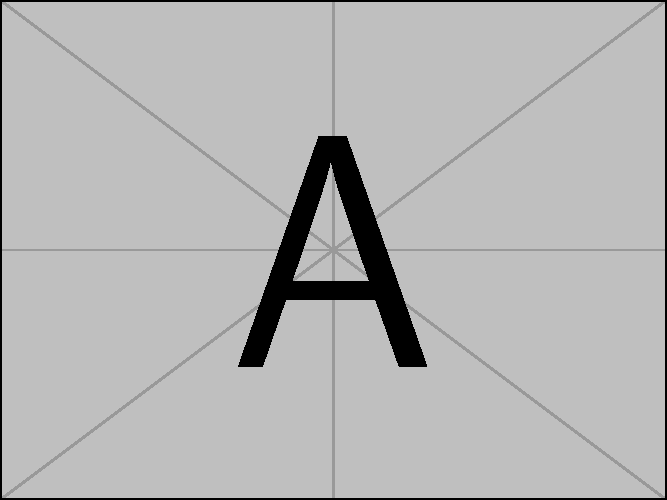
\includegraphics[width=0.5\linewidth]{example-image-a.pdf}
  \bifigcaption{图片示例\cite{TUN2025LaTeXThesisTe}}{Example Image\cite{TUN2025LaTeXThesisTe}}
  \label{fig:eg1}
\end{figure}

引用文献中的图\cite{TUN2025LaTeXThesisTe}时,除在正文文字中标注参考文献序号以外,还必须在中、
英文图题的右上角标注参考文献序号。

图中若有子图时,如\figref{fig:eg2}所示,子图题置于子图之下或图题之下,用中、英文书写,子图
号用a)、b)等表示。

\begin{figure}
  \centering
  \subcaptionbox{子图 A\protect\\ \thesubfigure\, Subfigure A\label{fig:subfig-a}}
    {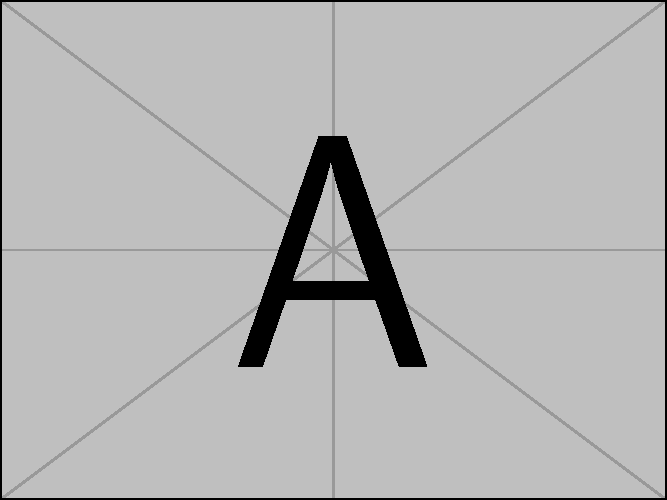
\includegraphics[width=0.35\linewidth]{example-image-a.pdf}}
  \subcaptionbox{子图 B\protect\\ \thesubfigure\, Subfigure B\label{fig:subfig-b}}
    {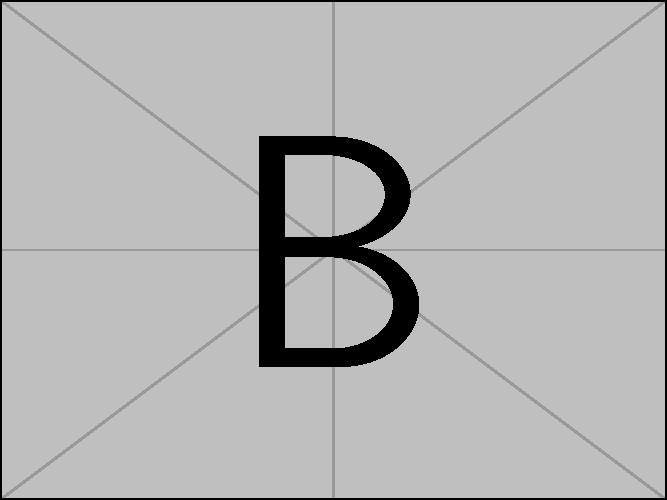
\includegraphics[width=0.35\linewidth]{example-image-b.pdf}}
  \bifigcaption{多个子图的示例}{Example of Multiple Subfigures}
  \label{fig:eg2}
\end{figure}

图中各部分说明应采用中文(引用的外文图除外)或数字符号,各项文字说明
置于图题之上(有子图时,置于子图题之上)。

图中文字用宋体(中文)或Times New Roman 字体(西文),字号尽量采用五号字(当字数较多时可用小五,以清晰表达为原则,但在一个插图内字号要统一)。同一图内使用文字应统一。

插图之前,文中必须有关于本插图的提示,如“见图1-1”、“如图1-1所示”
等。插图与其图题为一个整体,不得拆开排写于两页。插图处的该页空白不够排
写该图整体时,则可将其后文字部分提前排写,将图移到次页。有子图时,子图
过多在一页内安排不下时,可转到下页,总图题只出现在下页。

为了实现北京交通大学论文格式要求的双语图名,必须使用本文规定格式进行图片插入。以\figref{fig:eg1},\figref{fig:eg2}为例,对于*.pdf、*.jpg、*.png等格式图片插入代码格式为:

\begin{lstlisting}[language={[LaTeX]TeX}]
\begin{figure}[位置控制]
  \centering
  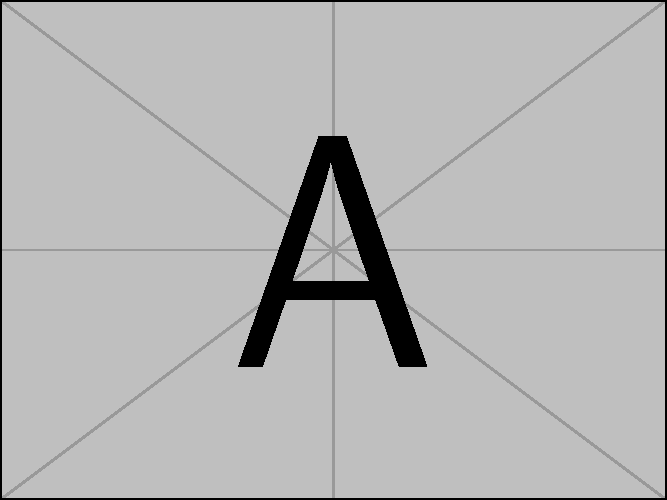
\includegraphics[显示宽度]{example-image-a.pdf(文件名)}
  \bifigcaption{中文图名}{英文图名}
  \label{标签名}
\end{figure}

\begin{figure}[位置控制]
  \centering
  \subcaptionbox{{子图中文图名1}\protect\\ \thesubfigure\, {子图英文图名1}\label{子图标签名1}}
    {\includegraphics[显示宽度]{文件名1}}
  \subcaptionbox{{子图中文图名2}\protect\\ \thesubfigure\, {子图英文图名2}\label{子图标签名2}}
    {\includegraphics[显示宽度]{文件名2}}
  \bifigcaption{总图中文名}{总图英文名}
  \label{总图标签名}
\end{figure}
\end{lstlisting}

\noindent 其中“[]”内可设置的属性字段请查阅\LaTeX{}的graphics宏包文档\cite{CP2024Packagesgraphi},此处不再赘述。

若插入*.svg格式的矢量图,则不可使用\cs{includegraphics}命令,如矢量\figref{猪肉刺身杯},其插入代码应修改为:

\begin{figure}[H]
  \centering
  \includesvg[width=7cm]{example-svg.svg}
  \bifigcaption{svg插入示例(Zeto设计)}{Example of svg (designed by Z.T. YEUNG)}
  \label{猪肉刺身杯}
\end{figure}

\begin{lstlisting}[language={[LaTeX]TeX}]
\begin{figure}[位置控制]
  \centering
  \includesvg[显示宽度]{svg文件名}
  \bifigcaption{中文图名}{英文图名}
  \label{标签名}
\end{figure}
\end{lstlisting}

\subsection{插表}
表应有“自明性”。表应有表题,表题即表的名称,置于表的编号之后。

表格不加左、右边线。表的编排建议采用国际通行的三线表,如\tabref{tab:eg1}。表中文字用宋
体(中文)或Times New Roman字体(英文),字号尽量采用5号字(当字数较多
时可用小5号字,但在一个插表内字号要统一)。 

表头设计应简单明了,尽量不用斜线。表头中可采用化学符号或物理量符号。 
全表如用同一单位,则将单位符号移至表头右上角,加圆括号。

表中数字空缺的格内加横线“—”(占2个半角字符)。表内文字或数字上、
下或左、右相同时,不允许用“〃”、“同上”之类的写法。 

表内文字说明,起行空2个半角字符,转行顶格,句末不加标点。

\begin{table}[H]\wuhao
  \centering
  \renewcommand\arraystretch{1.0} % 行距
  \bitabcaption{三线表示例\cite{TUN2025LaTeXThesisTe}}{Example Table\cite{TUN2025LaTeXThesisTe}}
  \begin{tabular}{ll}
    \toprule
    文件名          & 描述                         \\
    \midrule
    bjtumaster.cls   & 模板文件                     \\
    main.tex & 论文主文档    \\
    chapters & 论文章节存放目录  \\
    figures & 论文插图存放目录        \\
    betterbib.bib & 论文参考文献库(BibLaTeX)        \\
    gbt7714-numerical.bst & BibTeX 参考文献表国标样式文件    \\
    bibspacing.sty & 参考文献间距调整宏包  \\
    \bottomrule
  \end{tabular}
  \label{tab:eg1}
\end{table}

插表之前文中必须有相关文字提示,如“见表1-1”、“如表1-1所示”。一般
情况下插表不能拆开两页编排,如某表在一页内安排不下时,才可转页,以续表
形式接排。表右上角注明编号,编号后加“(续表)”,并重复表头,如\tabref{tab:eg2}所示。
插表的上下与文中文字间需空一行编排。 

引用文献中的表格时,除在正文\cite{TUN2025LaTeXThesisTe}文字中标注参考文献序号以外,还必须在中、
英文表题的右上角标注参考文献序号。

% 在 longtable 之前定义表清单标题(隐藏)
\begin{table}[H]
  \bitabcaption{跨页长表格}{Long Tables Across Pages}
  \label{tab:eg2}
\end{table}
\vspace{-1cm}
\addtocounter{table}{-1} % 回退表格计数器
\begin{longtable}{cccc}
    \toprule
    表头 1 & 表头 10 & 表头 11 & 表头 100 \\
    \midrule
  \endfirsthead
    \caption*{续表~\thetable\quad {跨页长表格}\vspace{-0.8cm}} \\
    \caption*{Continued Table~\thetable\quad {Long Tables Across Pages}} \\
    \toprule
    表头 1 & 表头 10 & 表头 11 & 表头 100 \\
    \midrule
  \endhead
    \bottomrule
  \endfoot
  Row 1  & & & \\
  Row 2  & & & \\
  Row 3  & & & \\
  Row 4  & & & \\
  Row 5  & & & \\
  Row 6  & & & \\
  Row 7  & & & \\
  Row 8  & & & \\
  Row 9  & & & \\
  Row A & & & \\
  Row B  & & & \\
  Row C  & & & \\
  Row D  & & & \\
  Row E & & & \\
  Row F & & & \\
  Row 10 & & & \\
  Row 11  & & & \\
  % Row 12  & & & \\
  % Row 13  & & & \\
  % Row 14 & & & \\
  % Row 15 & & & \\
  % Row 16 & & & \\
  % Row 17  & & & \\
  % Row 18  & & & \\
  % Row 19  & & & \\
  % Row 1A & & & \\
  % Row 1B & & & \\
  % Row 1C & & & \\
  % Row 1D  & & & \\
  % Row 1E  & & & \\
  % Row 1F  & & & \\
  % Row 20 & & & \\
\end{longtable}

本文非常不建议手搓表格代码,建议使用第三方插件如Create LaTeX tables online\cite{TabCreateLaTeXta}制作表格再拷贝进\LaTeX{}进行进一步处理,故不介绍普通表格插入命令。

若非不可抗力,尽量避免跨页长表格。对于跨页长表格,本模板为了实现中英文双语表题且在图清单内正常显示,采用了非常拙劣的办法。建议查看代码理解,具体步骤为:
\begin{enumerate}
    \item 使用\cs{begin\{table\}......}\cs{end\{table\}}定义一个双语表题(及标签)
    \item 使用\cs{vspace\{-1cm\}}减少表题与表格的间距
    \item 使用\cs{addtocounter\{table\}{-1}}回退表格计数器
    \item 使用\cs{begin\{longtable\}......}\cs{end\{longtable\}}定义跨页长表格。
\end{enumerate}
在第4)步中,需要再次输入一遍双语表题,具体修改部分为:

\begin{lstlisting}[language={[LaTeX]TeX}]
    \caption*{续表~\thetable\quad {中文表题}\vspace{-0.8cm}} \\
    \caption*{Continued Table~\thetable\quad {英文表题}} \\
\end{lstlisting}

在单元格内若需要进行换行操作,则需要使用\cs{makecell}宏包的指令,添加在需要换行的单元格上,如:

\begin{lstlisting}[language={[LaTeX]TeX}]
    \makecell{换行前的内容 \\ 换行后的内容}
\end{lstlisting}

\subsection{缩写、公式}

\subsubsection{缩写}
采用英语缩写词时,除本行业广泛应用的通用缩写词外,文中第一次出现的缩写词应该用括号注明英文原词。

\textbf{eg:} 自由度(Degree of Freedom, DoF)

\subsubsection{公式}
公式分为行内公式与行间公式两种。行内公式常用来表示简单物理量符号,不编号,有两种表示方法(后者不推荐),如“我们常用$\xi$表示机构局部自由度”的代码为:
\begin{lstlisting}[language={[LaTeX]TeX}]
我们常用$\xi$表示机构局部自由度
我们常用\(\xi\)表示机构局部自由度
\end{lstlisting}

行间公式可以使用\cs{equation}和\cs{equation*}环境,前者自动进行公式编号,后者不进行编号。若需要引用,则需要在公式开始后立即设置标签。
\vspace{2em}

\textbf{eg:}机构通用自由度公式\cite{HuangZhen2011LunJiGouZiYouDu}为:

\begin{equation}\label{自由度}
    M=d\left( n-g-1 \right) +\sum_{k=1}^g{f_k}+v-\xi
\end{equation}
式中,$d$为机构维数,$n$为构件数目,$g$为运动副数目,$\sum_{k=1}^g{f_k}$为各运动副自由度之和,$\xi$为局部自由度。

\equref{自由度}代码为:

\begin{lstlisting}[language={[LaTeX]TeX}]
\begin{equation}\label{自由度}
    M=d\left( n-g-1 \right) +\sum_{k=1}^g{f_k}+v-\xi =6\left( 5-4-1 \right) +4=4
\end{equation}
\end{lstlisting}

不编号行间公式亦可使用更快捷的\cs{[...}\cs{]或\$\$...\$\$}(后者不推荐)。

\textbf{eg:}空间任何一个矢量$\boldsymbol{s}$都可以由一个旋量$\textsl{\$}$来表达其方向和所在的空间位置\cite{GuoFang2007BingLianJiQiRenJiGouZongHeFangFaBiJiaoYanJiu},记作

\begin{equation*}
    \textsl{\$}=\left[  \begin{array}{c}
	               \boldsymbol{s}\\
	               \boldsymbol{s}_0+h\boldsymbol{s}\\
                    \end{array} \right] 
\end{equation*}

上式代码为:(论文中禁止使用“上式”、“上图”这种说法)
\begin{lstlisting}[language={[LaTeX]TeX}]
\begin{equation*}
    \textsl{\$}=\left[  \begin{array}{c}
	               \boldsymbol{s}\\
	               \boldsymbol{s}_0+h\boldsymbol{s}\\
                    \end{array} \right] 
\end{equation*}
或
\[
\textsl{\$}=\left[  \begin{array}{c}
	               \boldsymbol{s}\\
	               \boldsymbol{s}_0+h\boldsymbol{s}\\
                    \end{array} \right] 
\]
或
$$
\textsl{\$}=\left[  \begin{array}{c}
	               \boldsymbol{s}\\
	               \boldsymbol{s}_0+h\boldsymbol{s}\\
                    \end{array} \right] 
$$
\end{lstlisting}





较长的公式或多行公式需要转行时,应尽可能在“$=$”处回行,如\figref{自由度2},或者在“$+$”、“$-$”、“$\times$”、“$/$”等记号处对齐。

\begin{equation}\label{自由度2}
\begin{aligned}
    M &= d\left( n-g-1 \right) +\sum_{k=1}^g{f_k}+v-\xi \\
     &= 6\left( 5-4-1 \right) +4\\
     &= 4
\end{aligned}
\end{equation}

\equref{自由度2}代码为:

\begin{lstlisting}[language={[LaTeX]TeX}]
\begin{equation}\label{自由度2}
\begin{aligned}
    M &= d\left( n-g-1 \right) +\sum_{k=1}^g{f_k}+v-\xi \\
     &= 6\left( 5-4-1 \right) +4 \\
     &= 4
\end{aligned}
\end{equation}
\end{lstlisting}

公式中第一次出现的物理量代号应给予注释,注释的转行应与破折号“——”后第一个字对齐。破折号占4个半角字符,注释物理量需用公式表示时,公式后不应出现公式编号。

\subsection{算法、代码}

\subsubsection{算法}

算法环境使用\cs{algorithm}宏包,如\algref{alg1}的代码所示。

\begin{algorithm}
  \caption{Calculate $y = x^n$}
  \label{alg1}
  \small
  \begin{algorithmic}
    \REQUIRE $n \geq 0$
    \ENSURE $y = x^n$

    \STATE $y \leftarrow 1$
    \STATE $X \leftarrow x$
    \STATE $N \leftarrow n$

    \WHILE{$N \neq 0$}
      \IF{$N$ is even}
        \STATE $X \leftarrow X \times X$
        \STATE $N \leftarrow N / 2$
      \ELSE[$N$ is odd]
        \STATE $y \leftarrow y \times X$
        \STATE $N \leftarrow N - 1$
      \ENDIF
    \ENDWHILE
  \end{algorithmic}
\end{algorithm}

\subsubsection{代码}

代码提供行间代码与行内代码两种。行内代码适用场景较少,\\
如显示行内代码“\cs{input\{chapter03.tex\}}”的指令为:

\begin{lstlisting}[language={[LaTeX]TeX}]
\cs{input\{chapter03.tex\}}
\end{lstlisting}
\vspace{2em}
这是一段python代码,它作为行间代码显示在正文中:

\begin{lstlisting}[language={Python}]
def hello():
    print("Hello, World!")

hello()
\end{lstlisting}

显示这段python代码的指令为:

\begin{lstlisting}[language={[LaTeX]TeX}]
\begin{lstlisting}[language={Python}]
    def hello():
        print("Hello, World!")
    
    hello()
\end{lstlisting }
\end{lstlisting}

\subsection{引用}

\subsubsection{文献及电子资料}

论文中以任何形式引用的资料,均须标出引用出处,并以参考文献形式统一编号。引文标注遵照GB/T 7714-2005《文后参考文献著录规则\cite{QuanGuoXin2005WenHouCanKaoWenXianZhuLuGuiZe}》,采用顺序编码制。

当提及的参考文献为文中直接说明时,则用小4号字与正文排齐,如“由文献[2,4-7]可知”。

不得将引用文献标示置于各级标题处。

本文推荐采用BibLaTeX进行参考文献处理,即:对参考文献条目生成BibLaTeX格式的*.bib文件,将其内容拷贝至\cs{betterbib.bib}文件内。如文献管理软件Zotero可在安装betterbib插件后,在题录列表右键菜单内通过导出条目获得*.bib文件,如\figref{fig:zotero}所示。

\begin{figure}[htbp]
  \centering
  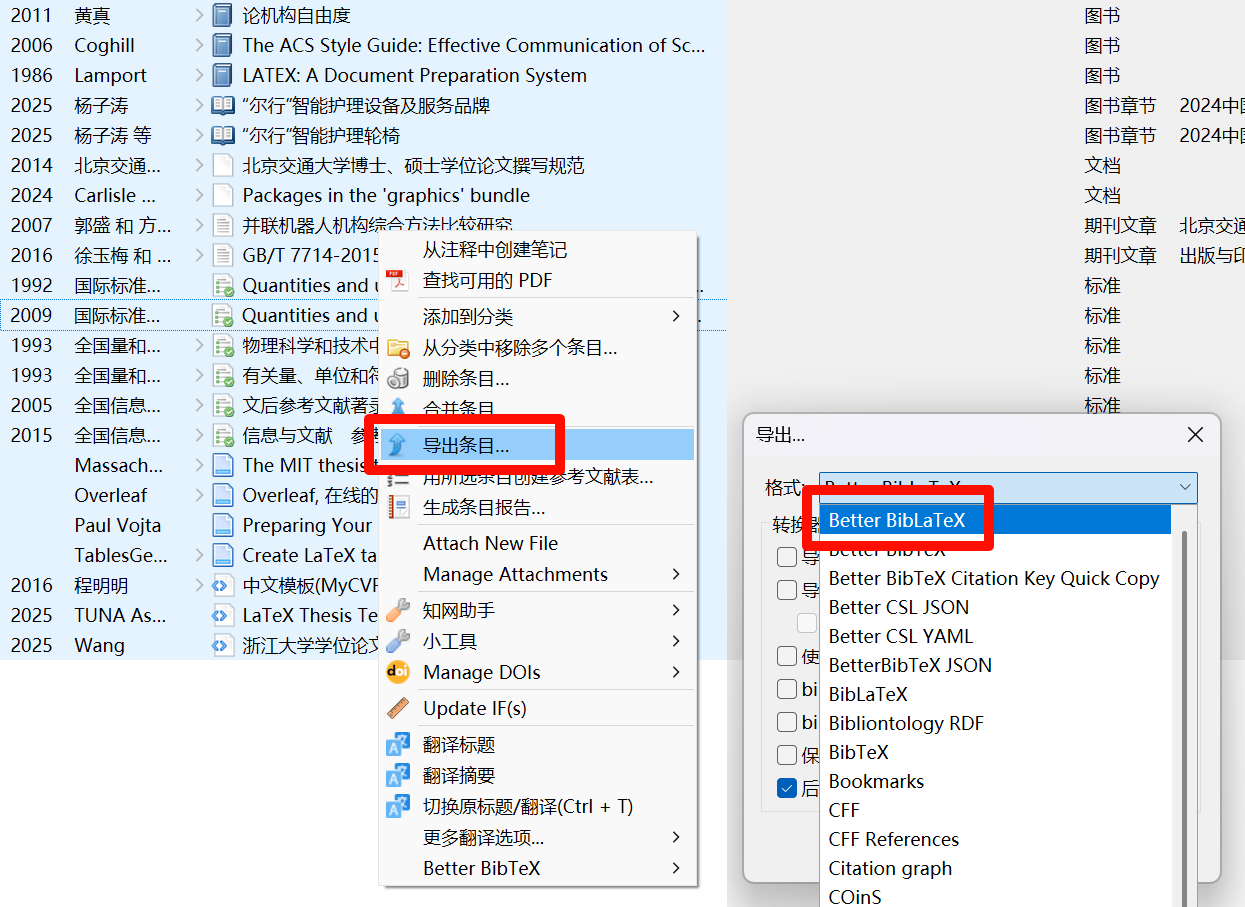
\includegraphics[width=0.8\linewidth]{figures/Zotero导出BibLaTeX流程.png}
  \bifigcaption{Zotero导出BibLaTeX流程}{The Process of Exporting BibLaTeX from Zotero}
  \label{fig:zotero}
\end{figure}

以《Sensing Expectation Enables Simultaneous Proprioception and Contact Detection in an Intelligent Soft Continuum Robot\cite{WXX+2024Sensingexpecta}》一文为例,其BibLaTeX代码为:

\begin{lstlisting}[language={BibTeX},keywordstyle={\color{Periwinkle}\bfseries}]
@article{WXX+2024Sensingexpecta,
  title = {Sensing Expectation Enables Simultaneous Proprioception and Contact Detection in an Intelligent Soft Continuum Robot},
  author = {Wang, Peiyi and Xie, Zhexin and Xin, Wenci and Tang, Zhiqiang and Yang, Xinhua and Mohanakrishnan, Muralidharan and Guo, Sheng and Laschi, Cecilia},
  date = {2024-11-18},
  journaltitle = {Nature Communications},
  shortjournal = {Nat Commun},
  volume = {15},
  number = {1},
  pages = {9978},
  publisher = {Nature Publishing Group},
  issn = {2041-1723},
  doi = {10.1038/s41467-024-54327-6},
  url = {https://www.nature.com/articles/s41467-024-54327-6},
  urldate = {2025-03-17},
}
\end{lstlisting}

在对参考文献进行引用时,在引用位置插入\cs{cite\{文献标签\}}即可。如引用上述文章的代码为:

\begin{lstlisting}[language={[LaTeX]TeX}]
    \cite{WXX+2024Sensingexpecta}
\end{lstlisting}

由于GB/T 7714-2005《文后参考文献著录规则\cite{QuanGuoXin2005WenHouCanKaoWenXianZhuLuGuiZe}》已经为过时标准,其替代标准为GB/T 7714-2015《信息与文献\quad 参考文献著录规则\cite{QuanGuoXin2015XinXiYuWenXianCanKaoWenXianZhuLuGuiZe}》,北京交通大学论文写作规范未及时更新,导致直接使用上述引用方法会有少许格式不符合学校规定。

新版本国家标准与旧版最主要的区别\cite{XuYu2016GB77142015YuGB}在于:新增了DOI号,新增了档案$[\mathrm{A}]$、舆图$[\mathrm{CM}]$、数据集$[\mathrm{DS}]$、其他$[\mathrm{Z}]$四类文献类型、用汉语拼音书写的中国著者不可缩写、标准名与标准号调换顺序、去除专利国别等。

\textbf{虽然变化如此之多,但视觉区别最大的是新增了DOI号。建议在Zotero导出前先删去“DOI号”字段(或修改gbt7714-numerical.bst文件)。同时建议对期刊、会议论文以及图书等非电子渠道独占资源删去“url”字段,虽符合旧国标与新国标,但有老师会觉得不顺眼,免得起争执。}

\subsubsection{论文内对图、表、公式、算法、章、节的引用}

在需要引用位置直接使用以下代码进行引用,不必手动输入“图”、“表”等字样:

\begin{lstlisting}[language={[LaTeX]TeX}]
    \figref{图片标签名}
    \tabref{表格标签名}
    \equref{公式标签名}
    \algref{算法标签名}
    \chptref{章标签名}
    \secref{节或子节标签名}
\end{lstlisting}

\subsubsection{脚注}

在需要脚注的位置直接使用以下代码进行脚注,每页最多10个(超过10个无法输入带圈数字\footnote{若要在其他地方输入带圈数字,可使用代码\cs{numcircled\{数字\}},该数字只能是1$\sim$10。}):

\begin{lstlisting}[language={[LaTeX]TeX}]
    \footnote{注释内容}
\end{lstlisting}


\clearpage
\section{数学符号规范}

中文论文的数学符号请务必规范处理。重点注意“标准字形”、“\textit{意大利字形}\footnote{\textit{意大利字形}(\textit{Italic Type})是拉丁字母字体排印学中的一种手写体印刷字形。因字形微向右倾斜,常被认为是西文斜体,但实际并非“斜体({\fontspec{XCharter}\hspace{-7em}\textsl{Slanting Type}})”。中文排印通常将\textit{楷体字形}与其建立对应关系。}”、“\textbf{增加字重字形}”三种字形在数学符号、上下标中的正确应用。

推荐参考GB/T 3102.11—1993《物理科学和技术中使用的数学符号\cite{QuanGuoLiang1993WuLiKeXueHeJiShuZhongShiYongDeShuXueFuHao}》、GB/T 3101—1993《有关量、单位和符号的一般原则\cite{QuanGuoLiang1993YouGuanLiangDanWeiHeFuHaoDeYiBanYuanZe}》与《The ACS Style Guide: CHAPTER 11 Numbers, Mathematics, and Units of Measure\cite{Cog2006ACSStyleGuide}》。其字形用法重点包括且不限于:

\subsection{{\kai 意大利字形(西文手写字形,对应中文楷体)}\textit{(Italic Type)}}  

\begin{enumerate}[label=(\arabic*)]
    \item \textbf{变量:} $T$代表温度,$x$代表分子分数,$r$代表速率
    \item \textbf{轴:} $y$ 轴
    \item \textbf{平面:}平面 $P$
    \item \textbf{矢量和张量的分量:} $a_x + b_x$
    \item \textbf{行列式和矩阵的元素:} $g_n$
    \item \textbf{常数:}$k_\mathrm{B}$,玻尔兹曼常数;$g$,重力加速度
    \item \textbf{描述变量的函数:}$f(x)$
    \item \textbf{定义传输属性的双字母变量:}$Kn$,Knudsen数;$Sr$,Strouhal数
\end{enumerate}


\subsection{\song 标准字形(罗马字形)(直体)(Roman Type)}

\begin{enumerate}[label=(\arabic*)]
    \item \textbf{数字}
    \item \textbf{标点符号和包围标记},如方括号、圆括号、大括号、绝对值符号等
    \item \textbf{大多数运算符},如加减乘除等号
    \item \textbf{缩写:}DoF,自由度;ARC,前交叉韧带
    \item \textbf{度量单位和时间单位:}mg,毫克;K,开尔文;Pa,帕斯卡;mmHg,毫米汞柱
    \item \textbf{非数学量或符号:} R,化学命名法中的自由基;$\mathrm{S_1}$,分子状态;s,原子轨道
    \item \textbf{变量的多字母缩写:} IP,电离电位;cmc,临界胶束浓度
    \item \textbf{数学常数:}e,自然对数的底数,2.71828...;i,虚数,$(-1)^{1/2}$;π,圆周率,3.14159...
    \item \textbf{矩阵的转置:} $\boldsymbol{A}^\mathrm{T}$($\mathrm{T}$ 是矩阵 $\boldsymbol{A}$ 的转置)
    \item \textbf{行列式:}$\mathrm{Det} \boldsymbol{A}$ 是矩阵 $\boldsymbol{A}$ 的行列式
    \item \textbf{三角函数和其他函数:}sin,lim,log,max,...
    \item \textbf{自定义运算规则:如坐标齐次变换}T()、R()、Tran()、Rot()
\end{enumerate}

\subsection{\song\textbf{增加字重字形(粗体)(Boldface Type)}}

\begin{enumerate}[label=(\arabic*)]
    \item \textbf{向量}
    \item \textbf{张量}
    \item \textbf{矩阵}
    \item \textbf{多维物理量:}$\mathbf{H}$,磁场强度
\end{enumerate}

\subsection{希腊字母(Ελληνικά Γράμματα)(Greek Letters)}
希腊字母(标准字形、\textbf{加粗字形}、\textit{意大利字形})可按字形要求用于变量、常量和向量等任何可使用拉丁字母的地方。

\subsection{Script字形(草书/书法体)与Open-Faced字形(空心/双线体)}
可以使用,但不推荐经常使用。常用的有:

\begin{enumerate}[label=(\arabic*)]
    \item \textbf{Script字形:}$\mathscr{L}$,拉格朗日量
    \item \textbf{Open-Faced字形:}$\mathbb{R}$,实数集
\end{enumerate}

\subsection{上标和下标(Subscripts and Superscripts)}

\begin{enumerate}[label=(\arabic*),itemsep=5pt]
    \item 对于本身就是物理量或数学符号的下标和上标,请使用\textit{意大利字形}。

            {\textbf{eg:\qquad }$C_p$ 表示恒压下的热容量。}

    \item 对于是缩写而不是符号的下标和上标,请使用标准字形(直体)。

            {\textbf{eg:\qquad }$C_\mathrm{B}$ 表示物体B的热容量。}
 
    \item 在大多数情况下,下标和上标最好错开。指数应放在下标之后。

            {\textbf{eg:\qquad }${C_x}^{1/2}$、$\Delta {H_1}^{\ddagger}$。\qquad 例外:$\mathrm{\lambda}_{+}^\infty$、$\mathrm{\sigma}_\mathrm{p}^+$、$B_2^{\mathrm{exptl}}$.}

    \item $\mathrm{e}^a$ 和 $\exp(a)$ 意义相同,可以互换。当以 $\mathrm{e}$ 为底数的指数很长或很复杂时,用 $\exp()$,将指数放在一行中用括弧标出。

            {\textbf{eg:\qquad }使用$\exp \left\{ \dfrac{1}{2}kT\left[ Y\left( a+b \right) -Z \right] \right\}$,避免使用$\mathrm{e}^{(1/2)kT\left[ Y\left( a+b \right) -Z \right]}.$}

    \item 在行文中,长公式避免使用根号而改用分数次幂。

            {\textbf{eg:\qquad }使用$\left[ \sinh ^2u+\left( \cosh u-1 \right) ^2 \right] ^{1/2}$,避免使用$\sqrt{ \sinh ^2u+\left( \cosh u-1 \right) ^2 }.$}
\end{enumerate}  % 第三章
\chapter{本地编译常见说明}

本模板本意为开发用于\overleaf 环境编译使用,但不排除有同学有本地编译需求或其它在线\LaTeX{}平台编译需求。特将几个在VSCode环境下编译报错重点以及修改方式进行说明。

\section{编译器Compiler错误导致编译失败}
本模板仅支持\XeTeX{} 编译器编译,不支持pdf\LaTeX{} 等旧时代编译器,请修改编译器设置(如通过修改VSCode的*.json文件。)

\section{字体问题}

\textbf{问题原因:}本模板采用\overleaf 平台内置的开源可商用字体。部分字体可能计算机本地未安装,因此无法编译。

\textbf{修复方法:}查看计算机已安装字体,并将\cs{bjtuthesis.cls}中的字体设置改为本地已有字体的名称。如将\cs{bjtuthesis.cls}中的280-289行从

\begin{lstlisting}[language={[LaTeX]TeX}]
    \setCJKmainfont[
  BoldFont = {Noto Serif CJK SC Bold},  % 主字体的增加字重字形
  ItalicFont = {AR PL UKai CN}  % 主字体的意大利字形
]{Noto Serif CJK SC}    % 主字体
\setCJKsansfont{Noto Sans CJK SC}   % 主无衬线字体
\setCJKmonofont{Noto Sans Mono CJK SC}  %主等宽字体
\setCJKfamilyfont{song}{Noto Serif CJK SC} % 宋体
\setCJKfamilyfont{hei}{Noto Sans CJK SC} % 黑体
\setCJKfamilyfont{fs}{cwTeXFangSong} % 仿宋
\setCJKfamilyfont{kai}{AR PL UKai CN} % 楷体
\end{lstlisting}

\noindent 直接修改为
\begin{lstlisting}[language={[LaTeX]TeX}]
    \setCJKmainfont[
  BoldFont = {宋体},  % 主字体的增加字重字形
  ItalicFont = {楷体}  % 主字体的意大利字形
]{宋体}    % 主字体
\setCJKsansfont{宋体}   % 主无衬线字体
\setCJKmonofont{黑体}  %主等宽字体
\setCJKfamilyfont{song}{宋体} % 宋体
\setCJKfamilyfont{hei}{黑体} % 黑体
\setCJKfamilyfont{fs}{仿宋} % 仿宋
\setCJKfamilyfont{kai}{楷体} % 楷体
\end{lstlisting}

可能导致显示效果不及预期,推荐使用思源宋体、更纱黑体等具有可变字重的字体以及开源可商用无版权风险的字体。(如常见的「微软雅黑」为不可商用的具有版权风险的字体。)

\section{*.svg格式的矢量图导致的编译错误}

\textbf{问题原因:}\secref{插图}一节中介绍了如何插入*.svg格式的矢量图,但其原理依旧是先将*.svg在内部转换为*.pdf再进行编译。部分编译环境如VSCode可能需要:

\begin{enumerate}[label=(\arabic*)]
    \item 修改*.json文件;
    \item 安装第三方插件;
    \item 将*.svg输出的*.pdf文件,其输出路径重定向指\cs{figure}目录在本地的绝对目录。
\end{enumerate}

\textbf{解决方法:}

方案一:建议将*.svg矢量图转换为*.pdf格式进行调用,避免直接调用*.svg矢量图。或直接转换为位图进行调用。均可正常进行编译。

方案二:对「问题原因」中所述的问题自行进行修复。  % 第四章


\cleardoublepage
\phantomsection
\vspace{-40pt}
\printbibliography[heading=bibintoc,title={参考文献}]


\bjtuappendix                               % 附录
\chapter{{\protect\\} \hspace{-13pt}{[补充内容]}}

本章内容参考《清华大学学位论文\LaTeX{}模板使用示例文档\cite{TUN2025LaTeXThesisTe}v7.5.1》。

附录是与论文内容密切相关、但编入正文又影响整篇论文编排的条理和逻辑
性的资料,例如某些重要的数据表格、计算程序、统计表等,是论文主体的补充内
容,可根据需要设置。

附录中的图、表、数学表达式、参考文献等另行编序号,与正文分开,一律用
阿拉伯数字编码,但在数码前冠以附录的序号,例如“图A-1”,“表A-1”,“式
(A-1)”等。

\section{插图}
如\figref{fig:app}所示,这是一张例图。

\begin{figure}[htbp]
  \centering
  
\includegraphics[width=0.8\linewidth]{bjtu_rrc.pdf}
  \bifigcaption{附录中的图片示例}{Example Image in Appendix}
  \label{fig:app}
\end{figure}

\noindent 例图结束。

\section{表格}
如\tabref{tab:app}所示,这是一张例表。

\begin{table}[H]\wuhao
  \centering
  \renewcommand\arraystretch{0.8} % 行距
  \bitabcaption{附录中的表格示例}{Example Table in Appendix}
  \begin{tabular}{ll}
    \toprule
    文件名          & 描述                         \\
    \midrule
    bjtumaster.cls   & 模板文件                     \\
    main.tex & 论文主文档    \\
    chapters & 论文章节存放目录  \\
    figures & 论文插图存放目录        \\
    betterbib.bib & 论文参考文献库(BibLaTeX)        \\
    gbt7714-numerical.bst & BibTeX 参考文献表国标样式文件    \\
    bibspacing.sty & 参考文献间距调整宏包  \\
    \bottomrule
  \end{tabular}
  \label{tab:app}
\end{table}

\section{数学表达式}

\begin{equation}\label{示例}
    M=d\left( n-g-1 \right) +\sum_{k=1}^g{f_k}+v-\xi 
\end{equation}

\equref{示例}是一个示例数学表达式,式中$d$为机构维数,$n$为构件数目,$g$为运动副数目,$\sum_{k=1}^g{f_k}$为各运动副自由度之和,$\xi$为局部自由度。


                  % 附录A

\chapter*{作者简历及攻读硕士学位期间取得的研究成果}
\markboth{作者简历及攻读硕士学位期间取得的研究成果}{}

\textbf{一、作者简历}

Zeto YEUNG,X,中国人,出生于千禧年。

\vspace{-10pt}

\begin{table}[H]
  \centering
  \renewcommand\arraystretch{0.8} % 行距
  \begin{tabular}{llll}
    2022.09$\sim$至今    & 北京交通大学 & 机械与电子控制工程学院 & 硕士研究生 \\
    2022.09$\sim$NOW    & BJTU & RRC, MECE & Master Student \\
  \end{tabular}
\end{table}

\textbf{二、发表论文}

\begin{enumerate}[label={[}\arabic*{]}]
	\item Yuki ASANO. Yuki ASANO的硕士生涯[Z]. 北京: 我家出版社, 2022: 22.
\end{enumerate}

\vspace{18pt}

\textbf{三、参与项目}

\begin{enumerate}[label={[}\arabic*{]}]
	\item 我家社会科学基金“面上”项目:《A Brown Fox Jumps over a Lazy Dog》,M2500000000
\end{enumerate}

\vspace{18pt}

\textbf{四、发明专利}

\begin{enumerate}[label={[}\arabic*{]}]
	\item Zeto YEUNG. 22$\sim$24岁的Zeto YEUNG: 我家,MH00222324[P].2025-02-25.
\end{enumerate}           % 个人简历、独创性声明
\chapter*{独创性声明}
\markboth{独创性声明}{}

本人声明所呈交的学位论文是本人在导师指导下进行的研究工作和取得的研究成果,除
了文中特别加以标注和致谢之处外,论文中不包含其他人已经发表或撰写过的研究成果,也
不包含为获得北京交通大学或其他教育机构的学位或证书而使用过的材料。与我一同工作的
同志对本研究所做的任何贡献均已在论文中作了明确的说明并表示了谢意。
\vspace{2cm}

{ 学位论文作者签名:\hspace{2cm} 签字日期:\hspace{1.5cm} 年\hspace{1cm} 月\hspace{1cm} 日}

\chapter*{学位论文数据集}
\markboth{学位论文数据集}{}
\begin{table}[H]
\caption*{表1.1: 数据集页}
\renewcommand\arraystretch{0.8} % 行距
\centering
	\begin{tabular}{|p{2.9cm}|p{2.1cm}|p{2.9cm}|p{3.4cm}|p{2.5cm}|}
		\hline	关键词* &密级* & 中图分类号 &	UDC& 论文资助\\
		\hline &&&&\\
		\hline	\multicolumn{2}{|l|}{学位授予单位名称*}&	学位授予单位代码*&	学位类别* & 学位级别*\\
		\hline	\multicolumn{2}{|l|}{北京交通大学}&	& & \\
		\hline	\multicolumn{2}{|l|}{论文题名*} &	\multicolumn{2}{l|}{并列题名}& 论文语种* \\
		\hline	\multicolumn{2}{|l|}{} &	\multicolumn{2}{l|}{}&\\
		\hline	作者姓名*&	\multicolumn{2}{l|}{}&学号* &\\
		\hline	\multicolumn{2}{|l|}{培养单位名称*}&培养单位代码*&培养单位地址&邮编\\
		\hline	\multicolumn{2}{|l|}{北京交通大学}&10004&	北京市海淀区西直门外上园村3号& 100044\\
        \hline	\multicolumn{2}{|l|}{学科专业*}&研究方向*&学制*&学位授予年*\\
        \hline	\multicolumn{2}{|l|}{}&&&\\
        \hline	论文提交日期*&\multicolumn{4}{l|}{}\\
		\hline	导师姓名*&\multicolumn{2}{l|}{}&职称*&\\
        \hline	评阅人&\multicolumn{2}{l|}{答辩委员会主席*}&\multicolumn{2}{l|}{答辩委员会成员}\\
        \hline	&\multicolumn{2}{l|}{}&\multicolumn{2}{l|}{}\\
               &\multicolumn{2}{l|}{}&\multicolumn{2}{l|}{}\\
        \hline \multicolumn{5}{|l|}{电子版论文提交格式  文本(~~)  图像(~~) 视频(~~) 音频(~~) 多媒体(~~) 其他(~~)}\\
        \multicolumn{5}{|l|}{推荐格式:application/msword;application/pdf}\\
        \hline	\multicolumn{2}{|l|}{电子版论文出版(发布)者}&\multicolumn{2}{l|}{电子版论文出版(发布)地}&权限声明\\
		\hline  \multicolumn{2}{|l|}{}&\multicolumn{2}{l|}{}&\\
		\hline  论文总页数*&\multicolumn{4}{l|}{}\\
		\hline  \multicolumn{5}{|l|}{共33项,其中带*为必填数据,为21项。}\\
		\hline
\end{tabular}
\end{table}

                  % 学位论文数据集



\end{document}              %%%%%%%%%%%%%%%%%%%%%%%%%%%%%% 论文结束
